\documentclass[11pt]{article}
\usepackage[T1]{fontenc}
\usepackage{lmodern}
\usepackage{amsmath,amssymb,amsthm}
\usepackage{graphicx}
\usepackage{booktabs}
\usepackage{microtype}
\usepackage[margin=0.92in]{geometry}
\usepackage{xcolor}
\usepackage[colorlinks=true,linkcolor=blue!55!black,citecolor=blue!55!black,urlcolor=blue!55!black]{hyperref}

\newtheorem{theorem}{Theorem}
\newtheorem{lemma}{Lemma}
\newtheorem{corollary}{Corollary}
\newcommand{\Bcal}{\mathcal B}
\newcommand{\Tcal}{\mathcal T}

\title{A Duhamel Formula for Continuously Forced Pantograph Equations}
\author{Candidate full-result packet for arXiv:1605.06734}
\date{26 August 2026}

\begin{document}
\maketitle

\begin{center}
\fbox{\parbox{0.91\textwidth}{
\textbf{Status: full solution likely valid; human review required.}
The formula below removes the source's analyticity restriction for the stated
first-order inhomogeneous pantograph equation and extends the scalar equation
to bounded operator coefficients on a Banach space.  The proof is complete.
Novelty confidence is moderate because an older equivalent Volterra-resolvent
formula may exist outside the bounded search.
}}
\end{center}

\section{Source target and exact scope}

The source is Cheng-shi Liu, \emph{Basic theory of a class of linear
functional differential equations with multiplication delay},
arXiv:1605.06734v4 \cite{Liu2016}.  (The manuscript title printed in the PDF is
\emph{Basic theory of a kind of linear pantograph equations}.)

At the transition from pp.~12 to 13, Section 4 says, in part:
\begin{quote}
``If non-homogenous term is a general smooth function, we do not know how to
solve the first order linear pantograph equation...''
\end{quote}
It then restricts Theorem 4.1 to analytic forcing in
\begin{equation}\label{eq:source}
 y'(x)=\beta y(\alpha x)+q(x),\qquad y(0)=a_0,
\end{equation}
and derives a Taylor-series formula.  The result in this packet answers that
specific general-smooth-forcing statement.  It does \emph{not} address the
paper's separate Open Problems 3.1 (exact zeros) or 5.1 (a variational
principle).

\begin{figure}[p]
\centering
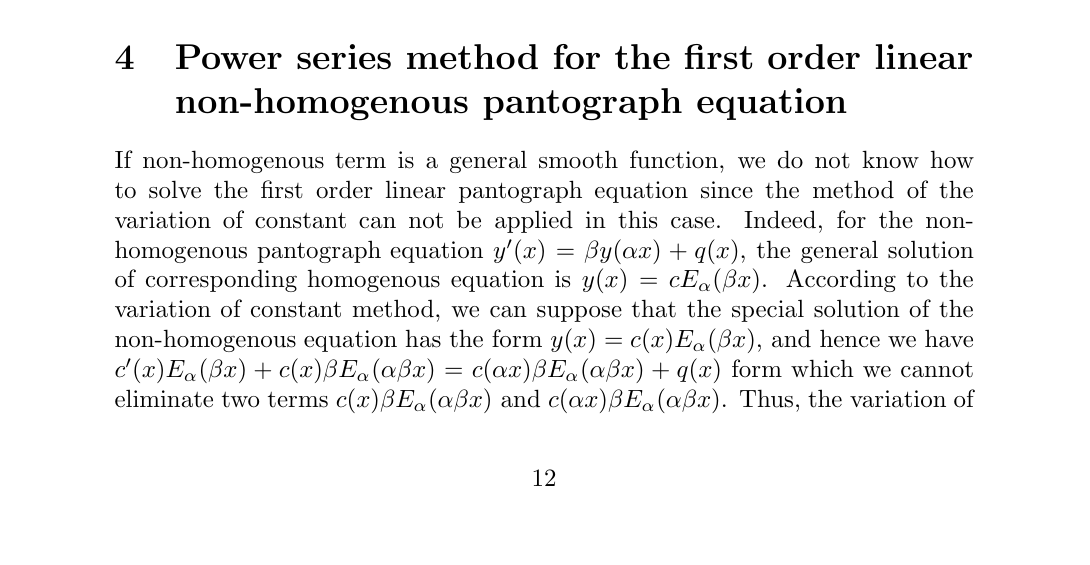
\includegraphics[width=\textwidth]{figures/open_problem_crop_page12.png}
\caption{Source p.~12: the assertion that general smooth forcing is not
handled by the scalar variation-of-constants ansatz.  The passage continues
on p.~13.}
\end{figure}

\begin{figure}[p]
\centering
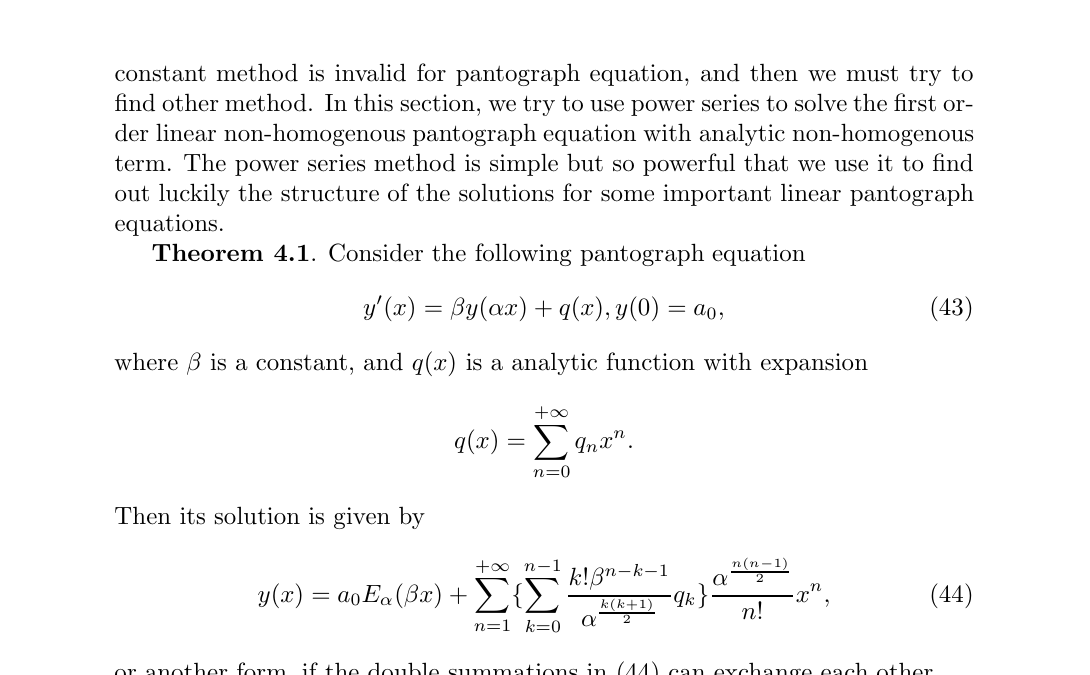
\includegraphics[width=\textwidth]{figures/open_problem_crop_page13.png}
\caption{Source p.~13: the continuation and Theorem 4.1, which assumes that
the forcing is analytic.}
\end{figure}

\section{Proof intuition}

The failed ansatz in the source tries to multiply the homogeneous solution by
a variable scalar.  The useful replacement is to integrate the equation once.
The delay then appears in the scaled Volterra operator
\[
 (\Tcal f)(x)=\int_0^x f(\alpha s)\,ds.
\]
Its iterates can be calculated exactly.  Besides the usual factorial decay of
a Volterra operator, the $n$th iterate gains the factor
$\alpha^{n(n-1)/2}$.  Thus $I-\Bcal\Tcal$ has a globally convergent Neumann
inverse on every compact interval, with no smallness assumption on the
coefficient.  Expanding this inverse against the initial constant and the
primitive of the forcing gives the formula below.

\section{The full result}

For a bounded operator $B$ on a Banach space $X$, write
\begin{equation}\label{eq:operatorE}
 E_\alpha(Bx)
 :=\sum_{n=0}^{\infty}
 \alpha^{n(n-1)/2}\frac{x^n B^n}{n!}.
\end{equation}
This series converges in operator norm for every real (indeed complex) $x$.
For $x<0$, every integral below is an oriented Bochner integral.

\begin{theorem}[Continuous-forcing pantograph resolvent]\label{thm:main}
Let $X$ be a real or complex Banach space, let $0<\alpha<1$, let
$B\in\mathcal L(X)$, let $q\in C(\mathbb R;X)$, and let $a\in X$.  There is a
unique $y\in C^1(\mathbb R;X)$ satisfying
\begin{equation}\label{eq:banach}
 y'(x)=B y(\alpha x)+q(x),\qquad y(0)=a.
\end{equation}
It is given by
\begin{equation}\label{eq:duhamel}
\boxed{
y(x)=E_\alpha(Bx)a+
\sum_{n=0}^{\infty}
\frac{\alpha^{n(n+1)/2}}{n!}B^n
\int_0^x (x-t)^n q(\alpha^n t)\,dt .
}
\end{equation}
The series converges absolutely and uniformly on every compact real interval.
\end{theorem}

\begin{proof}
Fix $R>0$ and work in $C([-R,R];X)$.  Define
\[
 (\Tcal f)(x):=\int_0^x f(\alpha s)\,ds.
\]
A direct induction, using oriented integrals when $x<0$, gives, for $n\geq1$,
\begin{equation}\label{eq:iterate}
 (\Tcal^n f)(x)=
 \frac{\alpha^{n(n-1)/2}}{(n-1)!}
 \int_0^x (x-t)^{n-1}f(\alpha^n t)\,dt.
\end{equation}
For completeness, suppose \eqref{eq:iterate} holds at $n$.  In
$\Tcal^{n+1}f$, substitute $u=\alpha t$ in the inner integral and exchange the
two integrations.  The substitution contributes $\alpha$, the polynomial
kernel contributes $\alpha^{n-1}$, and the final integration contributes
$1/n$.  Hence the coefficient is multiplied by $\alpha^n/n$, exactly changing
$\alpha^{n(n-1)/2}/(n-1)!$ into
$\alpha^{n(n+1)/2}/n!$.  The same computation on $[-R,0]$, or equivalently
the change $x\mapsto-x$, proves the oriented version.

In particular,
\begin{equation}\label{eq:Tbound}
 \|\Tcal^n f\|_{C([-R,R];X)}
 \leq \alpha^{n(n-1)/2}\frac{R^n}{n!}\|f\|_{C([-R,R];X)}.
\end{equation}
Let $\Bcal$ denote pointwise application of $B$.  The operators $\Bcal$ and
$\Tcal$ commute, so \eqref{eq:Tbound} implies norm convergence of
\[
 \sum_{n=0}^{\infty}(\Bcal\Tcal)^n
\]
on $C([-R,R];X)$, with no restriction on $R$ or $\|B\|$.

Set
\[
 Q(x)=\int_0^x q(t)\,dt,\qquad g(x)=a+Q(x).
\]
The differential equation \eqref{eq:banach} is equivalent to the integral
equation
\begin{equation}\label{eq:integral}
 y=g+\Bcal\Tcal y.
\end{equation}
Consequently its candidate solution is
\begin{equation}\label{eq:neumann}
 y=\sum_{n=0}^{\infty}(\Bcal\Tcal)^n g.
\end{equation}
The constant part satisfies
\begin{equation}\label{eq:constant}
 \Tcal^n a=\alpha^{n(n-1)/2}\frac{x^n}{n!}a.
\end{equation}
For the forcing part, \eqref{eq:iterate}, one more elementary Fubini
calculation, and the convention $\Tcal^0Q=Q$ give, for every $n\geq0$,
\begin{equation}\label{eq:forcingiterate}
 (\Tcal^nQ)(x)=
 \frac{\alpha^{n(n+1)/2}}{n!}
 \int_0^x (x-t)^n q(\alpha^n t)\,dt.
\end{equation}
Indeed, for $n\geq1$ insert
$Q(\alpha^n t)=\alpha^n\int_0^t q(\alpha^n u)\,du$ into
\eqref{eq:iterate}; integrating $(x-t)^{n-1}$ from $u$ to $x$ supplies the
factor $(x-u)^n/n$.  Formula \eqref{eq:forcingiterate} follows, again with the
same oriented identity on the negative half-line.

Substitution of \eqref{eq:constant} and \eqref{eq:forcingiterate} into
\eqref{eq:neumann} is exactly \eqref{eq:duhamel}.  If
$M_R=\sup_{|s|\leq R}\|q(s)\|$, the norm of its $n$th forcing term is bounded
uniformly for $|x|\leq R$ by
\begin{equation}\label{eq:forcebound}
 M_R R\,\frac{\alpha^{n(n+1)/2}(\|B\|R)^n}{(n+1)!}.
\end{equation}
This proves absolute compact-uniform convergence.  Equation
\eqref{eq:neumann} therefore satisfies \eqref{eq:integral}; since $q$ and $y$
are continuous, the right side of \eqref{eq:integral} is $C^1$ and
differentiation yields \eqref{eq:banach}.

It remains to prove uniqueness.  If $z$ is the difference of two solutions,
then $z=\Bcal\Tcal z$.  Iterating and using \eqref{eq:Tbound} gives
\[
 \|z\|_{C([-R,R];X)}
 \leq \alpha^{n(n-1)/2}\frac{(\|B\|R)^n}{n!}
 \|z\|_{C([-R,R];X)}
 \qquad(n\geq1).
\]
The scalar coefficient tends to zero.  Thus $z=0$ on $[-R,R]$.  Since $R$ was
arbitrary, uniqueness holds on all of $\mathbb R$.
\end{proof}

\section{Agreement with the source's analytic formula}

The following calculation is both a consistency check and the exact link to
Theorem 4.1 of the source.

\begin{corollary}\label{cor:source}
In the scalar case $B=\beta$, if
$q(x)=\sum_{k\geq0}q_kx^k$ is analytic, formula \eqref{eq:duhamel} has exactly
the Taylor coefficients displayed in equation (44) of arXiv:1605.06734v4.
\end{corollary}

\begin{proof}
The contribution of $q_k t^k$ to the $n$th forcing term is
\[
 \beta^n\alpha^{n(n+1)/2+nk}q_k
 \frac{k!}{(n+k+1)!}x^{n+k+1},
\]
because
\[
 \int_0^x(x-t)^nt^k\,dt
 =\frac{n!k!}{(n+k+1)!}x^{n+k+1}.
\]
Put $m=n+k+1$.  The exponent identity
\[
 \frac{n(n+1)}2+nk
 =\frac{m(m-1)}2-\frac{k(k+1)}2
\]
turns the coefficient of $x^m$ into
\[
 \frac{\alpha^{m(m-1)/2}}{m!}
 \sum_{k=0}^{m-1}
 \frac{k!\,\beta^{m-k-1}}{\alpha^{k(k+1)/2}}q_k,
\]
which is precisely the inhomogeneous coefficient in the source's formula
(44).  The homogeneous terms also agree by \eqref{eq:operatorE}.
\end{proof}

\section{Adversarial verification}

\subsection*{Step check}

\begin{center}
\begin{tabular}{@{}p{0.23\textwidth}p{0.12\textwidth}p{0.55\textwidth}@{}}
\toprule
Step & Verdict & Check \\
\midrule
Iterated kernel & Valid & Induction gives the factor
$\alpha^{n(n-1)/2}/(n-1)!$; exact monomial checks confirm the indices. \\
Neumann inversion & Valid & The bound \eqref{eq:Tbound} proves operator-norm
convergence on every compact interval even when $\|B\|R>1$. \\
Forcing kernel & Valid & Fubini yields \eqref{eq:forcingiterate}; the $n=0$
term is exactly $Q$. \\
Regularity & Valid & Compact-uniform convergence first gives the integral
equation; differentiability then follows from the Banach-valued fundamental
theorem of calculus, avoiding unjustified termwise differentiation. \\
Negative $x$ & Valid & Oriented integrals satisfy the same identities; the
equivalent substitution $x\mapsto-x$ changes $B,q$ to $-B,-q(-\cdot)$. \\
Uniqueness & Valid & Iterating the homogeneous integral equation and taking
$n\to\infty$ forces the compact sup norm to vanish. \\
Match to source & Valid & Corollary \ref{cor:source} recovers equation (44)
coefficient by coefficient. \\
\bottomrule
\end{tabular}
\end{center}

\subsection*{Computer guard checks}

The included script \texttt{code/verify\_formula.py} is not part of the proof.
It passed 961 exact exponent identities, 25 exact scalar Taylor coefficients,
38 exact components of a rational $2\times2$ matrix-coefficient test, and 41
high-precision residual tests on $[-2,2]$.  With 18 retained forcing terms,
the maximum residual was $2.3336307\times10^{-61}$ and the initial-value error
was zero.  From the packet directory, the command was:
\begin{quote}\small\ttfamily
conda run --no-capture-output -n sandbox python code/verify\_formula.py
\end{quote}

\section{Novelty check, limitations, and recommendation}

\paragraph{Bounded search.}
The four lightweight indexes for run \texttt{fa\_banach\_001} had no match for
the arXiv id or the continuous-forcing formula.  External searches used the
exact equation and combinations of \texttt{pantograph}, \texttt{Duhamel},
\texttt{variation of constants}, \texttt{Volterra resolvent}, and
\texttt{continuous forcing}.  The search also inspected the three works
returned by OpenAlex as citing arXiv:1605.06734, the TeX source of
arXiv:2303.09543 (which develops general successive approximation but does not
display \eqref{eq:duhamel}), and metadata/abstract material for classical and
recent generalized-pantograph work.  No occurrence of the explicit formula
\eqref{eq:duhamel} was identified.  This was a bounded search, not an
exhaustive priority claim.

\paragraph{Limitations.}
The theorem treats the pure proportional-delay equation in the source.  It
does not include a simultaneous undelayed term $A y(x)$ with noncommuting
operators, neutral terms involving $y'(\alpha x)$, variable dilation, or the
paper's unrelated zero and variational problems.  The assumption
$q\in C(\mathbb R;X)$ can be weakened to local Bochner integrability with an
almost-everywhere formulation, but that extension is not claimed here.

\paragraph{Recommendation.}
The mathematical verdict is \textbf{likely valid}, with high proof confidence.
Send to human review.  The primary mathematical check is the oriented-integral
calculation for $x<0$; the primary bibliographic check is whether an older
Volterra or pantograph source already contains the same explicit resolvent.

\begin{thebibliography}{9}
\bibitem{Liu2016}
C.-s. Liu,
\emph{Basic theory of a class of linear functional differential equations
with multiplication delay},
arXiv:1605.06734v4, 2018 revision; especially Section 4, pp.~12--14.
\end{thebibliography}

\end{document}
